\textbf{\textit{Detector Response and Statistical Treatment}}---
% The first step in our processing chain is to attain $\nu_{e}$, $\bar{\nu}_{e}$, and $\nu_{X}$ fluxes at the detector.
% These should take the form of the flux---in units of $\mathrm{MeV}^{-1}\,\mathrm{s}^{-1}\,\mathrm{cm}^{-2}$---as a function of energy at different points in time.
% These fluxes are then converted to hits in the IceCube detector using the \texttt{ASTERIA} package~\cite{ASTERIA}.
% In order to interface with this package, the tabulated fluxes must first be converted to a \texttt{SNEWPY}~\cite{SNEWS:2021ewj} model.
% This is done using the \texttt{Analytic3Species} model, which forgoes taking the tabulated flux as an input in favor of taking the expansion of the flux up to the third moment at each point in time.
% Our \texttt{ParameterizedFlux} class offers and interface between these parameters and the necessary portions of \texttt{SNEWPY} and \texttt{ASTERIA}.
% Additionally, we provide a convenience function, \texttt{parameterized\_flux\_from\_txt\_files} that automatically converts from tabulated fluxes stored in text files to a \texttt{ParametrizedFlux}.

% The parameters that \texttt{SNEWPY} takes in are assumed to describe the neutrino luminosity---the energy per unit time leaving the SN in neutrinos---at the source, and \texttt{SNEWPY} then handles oscillations before handing the final fluxes to \texttt{ASTERIA}.
% However, this is not desirable for BSM studies since the new effects may manifest in flight, and thus we typically wish to provide the flux at the detector.
% We circumvent this by taking advantage of the fact that \texttt{SNEWPY} uses the plane-wave approximation of a flux, reducing the magnitude of the flux by the the surface area of the sphere but otherwise neglecting the spherical geometry of neutrino front.
% This allows us to simulate a \textit{virtual supernova} near enough to the detector that oscillations will not play a role, scaling up the input flux by an appropriate amount to get a luminosity.
% Since at energies relevant to SNe, \textit{i.e.} between 1~MeV and 50~MeV, the smallest neutrino oscillation length is on the order of 100~m--50~km, we place the virtual supernova 1~m from the detector.
% We have tested the impact of using different lengths and, as expected, found no impact on our final sensitivities.

% \begin{figure}[t!]
%     \centering
%     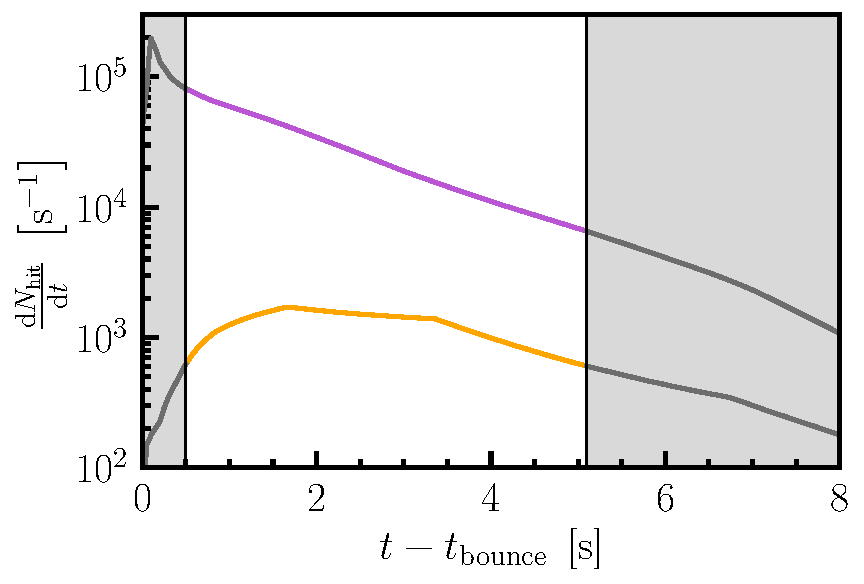
\includegraphics[width=0.47\textwidth]{figures/100MeV_HNL_hits-v-time.pdf}
%     \caption{\textbf{\textit{Hits versus time.}}}
%     \label{fig:hvt_100MeV}
% \end{figure}

% Having appropriately treated the flux at Earth, we can then take the number of hits created by the SM and neutrino fluxes as well as by the SM background, we may now turn to converting the hits to a sensitivity.
% In our study cases, the fluxes---and thus the hits in the detector---have different temporal profiles, see Fig.~\ref{fig:hvt_100MeV}.
% We then consider hits arriving within a certain time window defined by $t_{\mathrm{min.}}$ and $\Delta t$, where these times are measured relative to the so-called bounce time when the first neutrinos from the SN reach the detector.
% In practice, this time can be difficult to reconstruct, and so we consider time bins that are 0.1~s wide, well larger than the uncertainty on the SN start time.
% I NEED TO MAKE SURE THIS IS TRUE...
% We then consider the test given by:
% $$
% -2\log\mathcal{L} = 2\left[N_{\mathrm{exp.}} - N_{\mathrm{obs.}} + N_{\mathrm{obs.}} \log\left(\frac{N_{\mathrm{obs.}}}{N_{\mathrm{exp.}}}\right)\right]
% $$
% where $N_{\mathrm{exp.}}$ is the number of events expected from a given model and $N_{\mathrm{obs.}}$ is the number of neutrinos that would be observed in the SM only case.
% We then say that we are sensitive to a given model then this test statistic exceeds 3.841.
% See Fig.~\ref{fig:sensitivity_heatmap} for an example of the test statistic as a function of these two variables for two different models.

% \begin{figure}
%     \centering
%     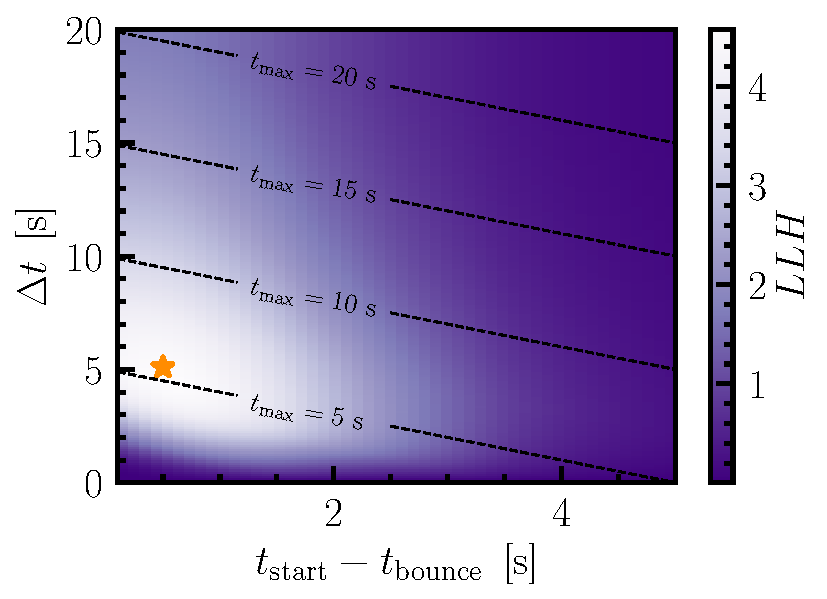
\includegraphics[width=0.47\textwidth]{figures/100MeV_sensitivity_heatmap.pdf}
%     \caption{\textbf{\textit{Test statistic as a function of $t_{\mathrm{start}}$ and $\Delta$t.}
%     }}
%     \label{fig:sensitivity_heatmap}
% \end{figure}